\subsection{Photoionization}

\begin{figure}[htbp]
    \centering
    \resizebox{\textwidth}{!}{
\begin{tikzpicture}[
  scale=0.62,
  well/.style      = {thick, black, line cap=round},
  ipline/.style    = {gray!70, thin},
  photonarr/.style = {photon,   line width=1.0pt, -{Stealth[length=5pt]}},
  elecarr/.style   = {electron, line width=1.1pt, -{Stealth[length=5pt]}},
  tick/.style      = {photon,   line width=1.0pt},
  panellabel/.style= {font=\small},
  regime/.style    = {font=\scriptsize, align=center, text width=2.8cm}
]

% étiquette -Ip (une seule fois, à gauche)
\node[font=\small] at (-2.65,-1) {$-I_p$};

% =====================================================================
% a) SINGLE-PHOTON  (xshift 0) : puits symétrique, flèche pleine
% Paramètre a = 0
% =====================================================================
\begin{scope}[xshift=0cm]
  \clip (-2.3,-2.05) rectangle (2.5,1.7);
  \draw[well] plot[domain=-2.5:-0.1, samples=50] (\x, {-1/(5*\x*\x) + 1});
  \draw[well] plot[domain=0.1:2.5, samples=50] (\x, {-1/(5*\x*\x) + 1});
  \draw[ipline] (-2.2,-1)--(2.2,-1);
  \draw[photonarr] (0,-1)--(0,1);
\end{scope}
\node[panellabel] at (-2.0,2.05) {a)};
\node[regime]     at (0,-2.75)   {single-photon\\ionization};

% =====================================================================
% b) ABOVE-THRESHOLD MPI  (x-shift 5) : même puits, flèche pointillée + rungs
% Paramètre a = 0
% =====================================================================
\begin{scope}[xshift=5cm]
  \clip (-2.3,-2.05) rectangle (2.5,1.7);
  \draw[well] plot[domain=-2.5:-0.1, samples=50] (\x, {-1/(5*\x*\x) + 1});
  \draw[well] plot[domain=0.1:2.5, samples=50] (\x, {-1/(5*\x*\x) + 1});
  \draw[ipline] (-2.2,-1)--(2.2,-1);
  % flèche pointillée
  \draw[photonarr] (0,-1.0)--(0,-0.5);
  \draw[photonarr] (0,-0.5)--(0,-0.0);
  \draw[photonarr] (0,0)--(0,0.5);
  \draw[photonarr] (0,0.5)--(0,1.0);
  

\end{scope}
\node[panellabel] at (3.0,2.05) {b)};
\node[regime]     at (5,-2.75)  {above-threshold\\multi-photon ionization};

% =====================================================================
% c) NON-ADIABATIC TUNNEL  (xshift 10) : barrière large, montée + tunnel
% Paramètre a = 0.1
% =====================================================================
\begin{scope}[xshift=10cm]
  \clip (-2.3,-2.05) rectangle (2.5,1.7);
  \draw[well] plot[domain=-2.5:-0.1, samples=50] (\x, {-1/(5*\x*\x) + 1 - 0.5*\x});
  \draw[well] plot[domain=0.1:2.5, samples=50] (\x, {-1/(5*\x*\x) + 1 - 0.5*\x});
  \draw[ipline] (-2.2,-1)--(2.2,-1);
  % montée multiphotonique (courte, jaune)
  \draw[photonarr] (0,-1.0)--(0,-0.5);
  \draw[photonarr] (0,-0.5)--(0,-0.0);
  % tunnel à travers la barrière (vert, sortie à droite)
  \draw[elecarr] (0,-0)--(2.60,-0);
\end{scope}
\node[panellabel] at (8.0,2.05)  {c)};
\node[regime]     at (10,-2.75)  {non-adiabatic\\tunnel ionization};

% =====================================================================
% d) ADIABATIC TUNNEL  (xshift 15) : barrière plus inclinée, tunnel à -Ip
% Paramètre a = 0.9
% =====================================================================
\begin{scope}[xshift=15cm]
  \clip (-2.3,-2.05) rectangle (2.5,1.7);
  \draw[well] plot[domain=-2.5:-0.1, samples=50] (\x, {-1/(5*\x*\x) + 1 - 1.9*\x});
  \draw[well] plot[domain=0.1:2.5, samples=50] (\x, {-1/(5*\x*\x) + 1 - 1.9*\x});
  \draw[ipline] (-2.2,-1)--(2.2,-1);
  % tunnel horizontal au niveau -Ip
  \draw[elecarr] (0,-1)--(2.25,-1);
\end{scope}
\node[panellabel] at (13.0,2.05) {d)};
\node[regime]     at (15,-2.75)  {adiabatic\\tunnel ionization};

% =====================================================================
% e) OVER-BARRIER  (xshift 20) : barrière abaissée sous -Ip, sortie libre
% Paramètre a = 1.6
% =====================================================================
\begin{scope}[xshift=20cm]
  \clip (-2.3,-2.05) rectangle (2.5,1.7);
  \draw[well] plot[domain=-2.5:-0.1, samples=50] (\x, {-1/(5*\x*\x) + 1 - 2.8*\x});
  \draw[well] plot[domain=0.1:2.5, samples=50] (\x, {-1/(5*\x*\x) + 1 - 2.8*\x});
  \draw[ipline] (-2.2,-1)--(2.2,-1);
  % l'électron passe au-dessus de la barrière supprimée
  \draw[elecarr] (0.0,-1)--(2.30,-1);
\end{scope}
\node[panellabel] at (18.0,2.05) {e)};
\node[regime]     at (20,-2.75)  {over-barrier\\ionization};

\end{tikzpicture}
}
    \caption{Illustration of the different ionization regimes.}
    \label{fig:regimes_ionisation}
\end{figure}

Strong focusing leads to a high optical intensity in the material. This strong concentration of photons at the same location increases the probability of multiphoton ionization, a nonlinear effect~\cite{mao2004}. The more intense the field, the more the potential binding the electron to the ion is deformed. Beyond a certain intensity threshold, the barrier takes a triangular shape and becomes thin enough to allow tunnel ionization. The Keldysh parameter was introduced to distinguish between the regime dominated by multiphoton ionization and the regime dominated by tunnel ionization~\cite{mao2004}.

In the semiclassical model, an electron escapes through a barrier of width $l = U_i/e\mathcal{E}$ with a velocity $v = \sqrt{2U_i/m}$. The time needed to cross this distance is:
\begin{equation}
\tau_{\text{tun}} = \frac{l}{v} = \frac{U_i/e\mathcal{E}}{\sqrt{2U_i/m}} = \frac{\sqrt{2m U_i}}{e\mathcal{E}}
\end{equation}

The characteristic time during which tunnel ionization can occur is given by $\tau \approx 1/\omega_0$. The ratio of these two times is then:
\begin{equation}
\gamma = \frac{\tau_{\text{tun}}}{\tau} = \omega_0\frac{\sqrt{2m U_i}}{e\mathcal{E}}
\end{equation}

If the ratio $\gamma \ll 1$, the tunnel crossing time is very short compared to the ionization time. Tunnel ionization is then instantaneous on the scale of the laser cycle, and the field behaves as a quasi-static field. Conversely, if $\gamma \gg 1$, the field oscillates too fast for the electron to cross the barrier by tunneling, and ionization then requires multiphoton absorption~\cite{bulgakova2010}.

The Keldysh photoionization rate is defined as follows:
\begin{equation}
W_{PI}(|\mathcal{E}|) = \frac{2\omega_0}{9\pi}\bigg(\frac{\omega_0m}{\hbar\sqrt{\gamma_1}}\bigg)^{\frac{3}{2}}Q(\gamma,x)\exp(-\alpha\lceil x+1\rceil)
\end{equation}

With $\gamma_1 = \frac{\gamma^2}{1+\gamma^2}$, $\gamma_2 = \frac{1}{1+\gamma^2}$ and $x = \frac{2}{\pi}\frac{U_iE(\gamma_2)}{\hbar\omega_0\sqrt{\gamma_1}}$
\begin{equation}
Q(\gamma,x) = \frac{\pi}{2K(\gamma_2)}\sum^\infty_{n=0}\exp \bigg(-n\pi\frac{K(\gamma_1)-E(\gamma_1)}{E(\gamma_2)}\bigg)\Phi\bigg(\frac{\pi}{2}\sqrt{\frac{n+2\lceil x + 1\rceil-2x}{K(\gamma_2)E(\gamma_2)}}\bigg)
\end{equation}

$\Phi$ is the Dawson function $\Phi(z) = e^{-z^2}\int^z_0e^{y^2}dy$ and $K$ and $E$ are respectively the complete elliptic integrals of the first and second kind, with the parameter $m = k^2$
\begin{align}
K(m) &= \int_0^{\pi/2} [1 - m \sin(t)^2]^{-1/2} dt \\
E(m) &= \int_0^{\pi/2} [1 - m \sin(t)^2]^{1/2} dt
\end{align}

As observed in reference~\cite{PhysRevB.71.125435}, filamentation in fused silica typically occurs at intensities around $5 \times 10^{13} \text{ W/cm}^2$, where multiphoton and tunnel ionization both contribute significantly.

\begin{figure}[htbp]
    \centering
    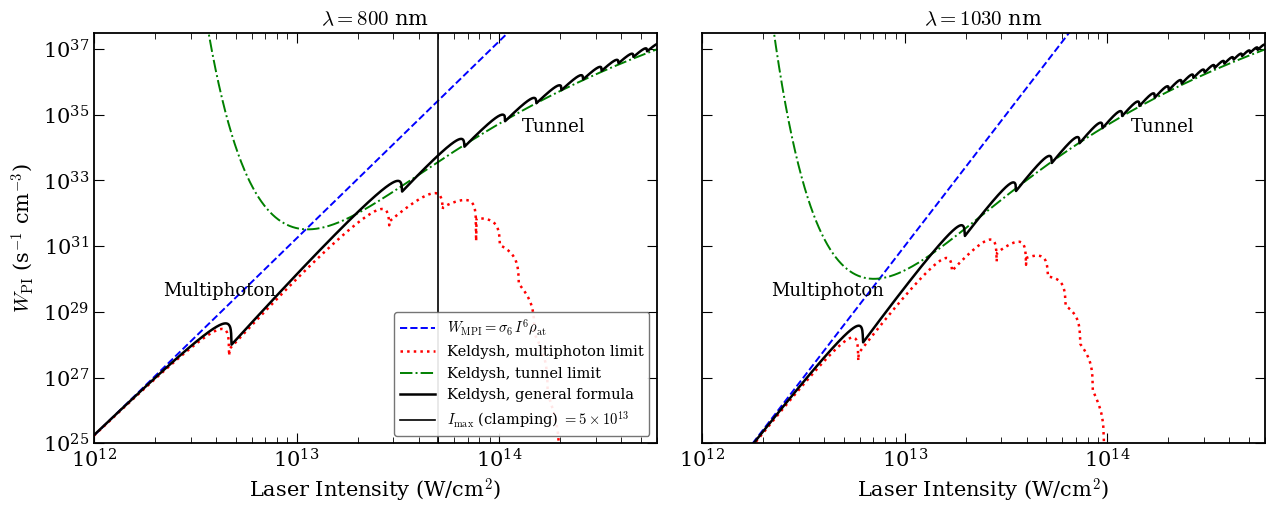
\includegraphics[width=1\linewidth]{sections/tlchargement.png}
    \caption{The photoionization rate $W_{\text{PI}}$ in fused silica ($U_i = 9 \text{ eV}$) is plotted against laser intensity for $\lambda = 800 \text{ nm}$ and $\lambda = 1030 \text{ nm}$. The solid black line represents the full general Keldysh formula, while the dotted red and dash dotted green lines show its exact analytical asymptotes for the multiphoton limit ($\gamma \gg 1$) and the tunnel limit ($\gamma \ll 1$) respectively. The dotted blue line corresponds to the standard perturbative MPI law ($W_{\text{MPI}} = \sigma_K I^K \rho_{\text{at}}$). The vertical gray line indicates the typical clamping intensity level ($\sim 5 \times 10^{13} \text{ W/cm}^2$) reached in filamentation simulations at 800 nm.}
    \label{fig:placeholder}
\end{figure}
